\documentclass[report, backcover, french, nodocumentinfo]{upmethodology-document}
\usepackage[utf8]{inputenc}
\usepackage[T1]{fontenc}
%\usepackage{natbib}
\usepackage{csquotes}
%\usepackage[backend=biber,style=alphabetic,citestyle=authoryear]{biblatex}
\usepackage{amsmath}
\usepackage{amssymb}
\usepackage{hyperref}
\usepackage{listings}
\usepackage{textcomp}
\usepackage{color}
\usepackage[toc,page]{appendix}
\usepackage{wrapfig}
\usepackage{stackengine}
\usepackage{scalerel}

%link option, especialy for the table of contents
\hypersetup{
    colorlinks=true,
    linkcolor=black,
    urlcolor=blue,
    linktoc=all
}

\setfrontcover{classic}

\declaredocument{Conception de projet: clone de MiniMetro}{Rapport LO43}{LO43-A2016}
\setpublisher{Université de Technologie de Belfort-Montbéliard}

%\incversion{\makedate{jj}{mm}{aaaa}}{Initial version.}{\upmpublic}
\incversion{\today}{Initial version.}{\upmpublic}

\addauthorvalidator*[julien.barbier@utbm.fr]{Julien}{BARBIER}{Auteur original}
\addauthorvalidator*[maxime.pinard@utbm.fr]{Maxime}{PINARD}{Auteur original}

\addinformed*[franck.gechter@utbm.fr]{Franck}{GECHTER}{Professeur de l'UV LO43}

\setdockeywords{UTBM, LO43, MiniMetro, Java, JavaFX, UML}

\setcopyrighter{Julien BARBIER et Maxime PINARD}
\setpublisher{Julien BARBIER et Maxime PINARD}
\setprintingaddress{France}

%\setfrontcover{modern}
%\setfrontillustration[0.6]{figures/logo}

\graphicspath{./figures/}

%\bibsize{\normalfont}

\newcommand*\cleartoleftpage{%
  \clearpage
  \ifodd\value{page}\hbox{}\newpage\fi
}

\newcommand{\p}[1]{\paragraph{#1\\}}

%Function to print a warning sign
\newcommand{\dangersign}[1][2.5ex]
	{\renewcommand{\stacktype}{L}
		{\scaleto{\stackon[1pt]{\color{red}$\triangle$}{\fontsize{4pt}{4pt}\selectfont !}}{#1}}}

% For more information about UPmethodology: https://www.ctan.org/pkg/upmethodology

\begin{document}

	\upmdocumentsummary{}
	\upmdocumentauthors{}
	\upmdocumentinformedpeople{}
	\upmpublicationpage{}

	\tableofcontents{}
	\listoffigures{}

	\newpage{}
	\chapter{Rappel sur le projet}
		\p{}
			Nous devions réaliser dans le cadre de l'uv de LO43 un clone de Mini Metro. Pour ce faire nous avions fait un rapport intermédiaire pour présenter la conception du projet et ce rapport a été écrit pour présenter l'implémentation de celui-ci. Ainsi le but était d'avoir les mêmes fonctionnalités que Mini Metro a savoir :
			\begin{itemize}
				\item Gestion de Lignes
				\item Gestion de Trains
				\item Path-Finding pour les passagers
				\item Apparition de stations en fonction du Temps
			\end{itemize}
			On présentera donc les changements appliquées dans la conception, puis les fonctionnalités et nous terminerons par les implémentations futures
	\chapter{Conception et changement dans la conception}
		\section{Précision...}
			\p{}
			Durant le projet, nous avons respecté notre conception. Ainsi les changements furent plus de l'ordre des attributs et des méthodes. Les plus grands bouleversement se situe dans la vue.
		\section{Vue}
			\p{}
			La vue a été grandement remanié dans ce projet pour pouvoir l'adapter à JavaFx. Nous avions décidé d'utiliser JavaFx par le fait qu'il soit plus moderne que Swing et possède plus de fonctionnalité graphique que ce dernier. Mais il s'est révélé que JavaFx est relativement buggé, ce qui provoque de véritables difficulté pour l'implémentation de la vue. Il s'est révélé aussi magique dans le sens que les fonctions ne font pas forcément ce qu'elle doit faire. De plus, quand la fenêtre est rétréci, JavaFx fait de l'optimisation mal venu et provoque ensuite une liste d'exception ``JavaFx.NullPointerException'' car il a supprimé des éléments qui maintenant n'existe plus. Certains freeze ou autres problèmes graphiques peuvent venir de JavaFx et est ainsi indépendant de notre vonlonté.
			\p{}
			Néanmoins, la partie graphique marche sans réelle problème. Nous obtenons le diagramme de Classe \ref{fig:ViewDiagramm}.
			\begin{figure}[h!]
				\centering
				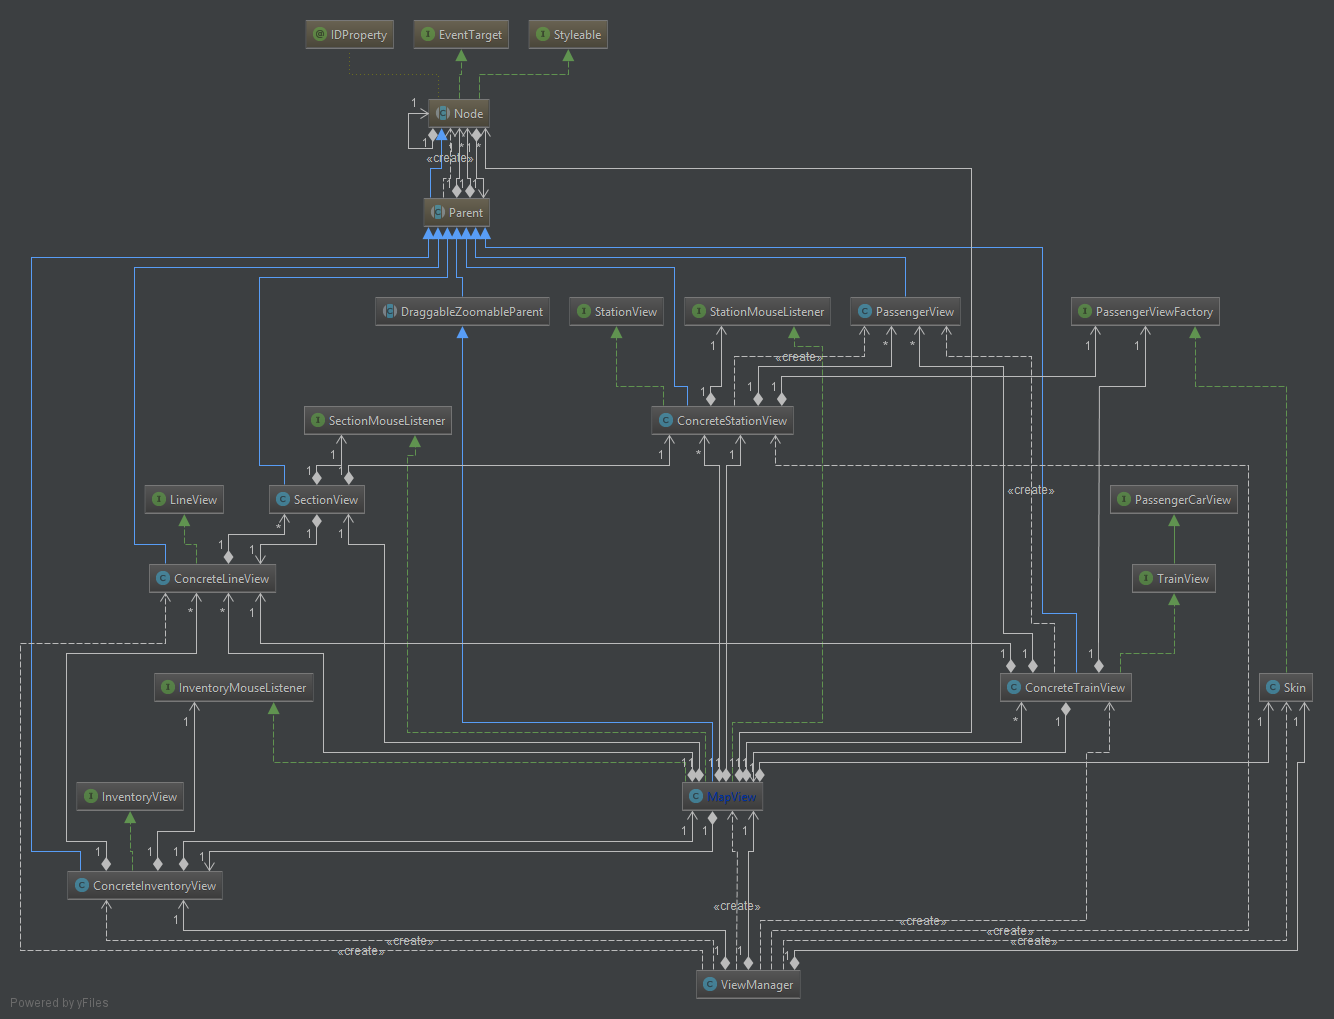
\includegraphics[width=\textwidth]{figures/ViewClassDiagrammFinal.png}
				\caption{Diagramme de la vue à la fin du Projet}
				\label{fig:ViewDiagramm}
			\end{figure}
			Comme on peut le voir, toute les classes à l'exception du ViewManager et de Skin héritent de Parent pour pouvoir les rajoutées dans la liste de Node de JavaFx. On retrouve les classes ConcreteXxxxView implémentent les interfaces leurs correspondant pour avoir une liaison Modèle vers Vue. Ainsi le modèle ne possèdent que l'interface et l'implémentation de cette interface dépendra de la lib graphique qu'on utilisera.

			TODO : continuez la présentation de la vue.
		\section{Modèle}
			TODO : explication de certaines fonction (Path-Finding)
	\chapter{Fonctionnalité présents dans le projet}
		\p{}
		Les fonctionnalités que nous avons réussi à implémenter dans les temps sont les suivantes : 
		\begin{itemize}
			\item Gestion des Lignes et présences de plusieurs ligne.
			\item Création de différentes Map
			\item Ajout de Train
			\item Apparition de station en fonction du temps
			\item Path-Finding pour les passengers
			\item Upgrade des stations (Bonus)
			\item Choix de Bonus tous les X temps.
		\end{itemize}
	\chapter{Fonctionnalité à Implémenter}
		\p{}
		Faute de temps, nous n'avons pas réussi à implémenter ces fonctionnalités : 
		\begin{itemize}
			\item Gestion des Wagons (Pour la vue du moins)
			\item Retrait de Train d'une ligne
			\item Loopage des trains
		\end{itemize}
	\chapter{Conclusion}
		\p{}
\end{document}